% !TEX encoding = UTF-8
% !TEX TS-program = pdflatex
% !TEX root = ../tesi.tex

%**************************************************************
\chapter{Progettazione e codifica}
\label{cap:progettazione-codifica}
%**************************************************************

\intro{In questo capitolo verranno spiegate le tecnologie utilizzate per lo sviluppo e l'architettura del prodotto software}\\

%**************************************************************
\section{Tecnologie e strumenti}
\label{sec:tecnologie-strumenti}

Di seguito viene data una panoramica delle tecnologie e strumenti utilizzati per lo sviluppo.

\subsection{Tecnologie}

\subsubsection*{Vue.js}
Vue.js è un framework javascript opensource nato nel 2013 che presenta un'architettura adottabile in modo incrementale che si concentra sulla composizione dei componenti, inoltre sono presenti funzionalità avanzate offerte tramite librerie e pacchetti di supporto. I componenti Vue estendono gli elementi HTML di base per incapsulare del codice riutilizzabile quindi a livello generale i componenti sono elementi personalizzati a cui il compilatore Vue associa una particolare funzionalità.\\
Vue utilizza quindi una sintassi basata su HTML e consente di associare il DOM renderizzato ai dati dell'istanza di Vue sottostante. In questo modo i modelli Vue possono essere analizzati da browser e parser HTML conformi alle modifiche ed inoltre con il sistema di reattività Vue è in grado di calcolare il numero minimo di componenti per eseguire nuovamente il rendering applicando la quantità minima di manipolazioni DOM quando cambia lo stato dell'app.

\subsubsection*{Vuetify}
Vuetify è un framework UI completo costruito su Vue.js nel 2014 ed il suo obiettivo è fornire agli sviluppatori gli strumenti per poter creare esperienze utente ricche e coinvolgenti. A differenza di altri framework Vuetify è progettato da zero in modo tale da renderlo facile da imparare ed essere gratificante da padroneggiare con centinaia di componenti realizzate dalle specifiche di Material Design.\\
Un pregio di questo framework è che adotta un approccio al mobile, questo significa che la web application sviluppata tramite esso sarà pienamente utilizzabile immediatamente su un tablet, un telefono ed un computer. Inoltre è un framework in sviluppo attivo che viene aggiornato settimanalmente rispondendo ai problemi e relativi report della community. Un altro pregio è, come si può vedere nell'immagine sottostante, il gran numero di funzionalità che possiede Vuetify in confronto agli altri framework di Vue.
\begin{figure}[h]
	\begin{center}
		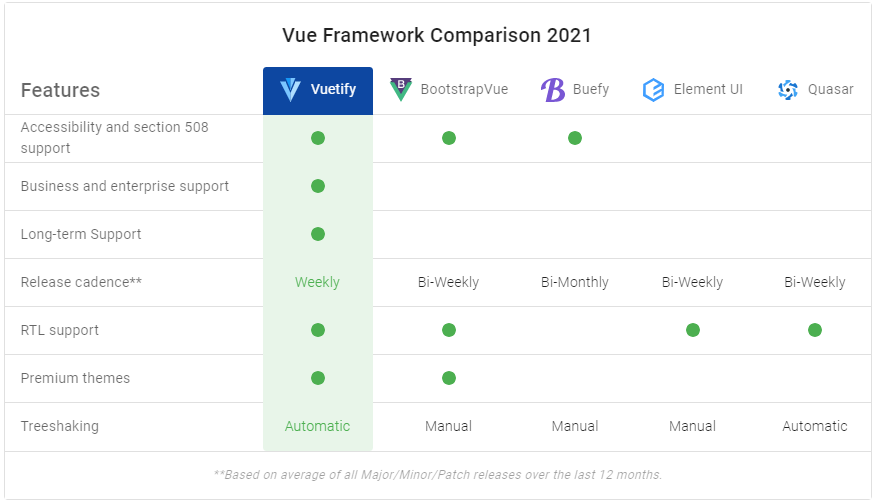
\includegraphics[width=1\columnwidth]{vuetify.png}
		\caption{Funzionalità di Vuetify}
	\end{center}
\end{figure}

\subsection{Strumenti}

\subsubsection{Github}

\subsubsection{Visual Studio Code}

%**************************************************************
\section{Ciclo di vita del software}
\label{sec:ciclo-vita-software}

%**************************************************************
\section{Progettazione}
\label{sec:progettazione}

\subsubsection{Namespace 1} %**************************
Descrizione namespace 1.

\begin{namespacedesc}
    \classdesc{Classe 1}{Descrizione classe 1}
    \classdesc{Classe 2}{Descrizione classe 2}
\end{namespacedesc}


%**************************************************************
\section{Design Pattern utilizzati}

%**************************************************************
\section{Codifica}
